\chapter{ANÁLISIS Y DISCUSIÓN DE RESULTADOS}
\section{Metadata}
Luego de 27 épocas, con un rango entre 2 y 3 segundos de entrenamiento cada una, el modelo dejó de entrenar dado que durante 7 épocas no registró una reducción en el valor de la pérdida del subconjunto de validación, por más que 3 épocas antes se había reducido su tasa de aprendizaje.

Así, de acuerdo a las Figuras \ref{5:fig1} y \ref{5:fig2}, en la época 20 se registran los mejores valores de exactitud y pérdida para el subconjunto de validación, alcanzando 0.9523 y 0.1246 respectivamente.

\begin{figure}[htbp]
	\begin{center}
		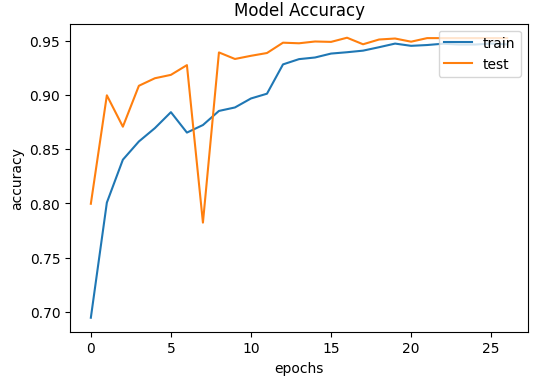
\includegraphics[width=0.60\textwidth]{4/figures/metadata_model_accuracy.png}
		\caption{Evolución de la exactitud de los subconjuntos de entrenamiento y validación para el modelo MLP de metadata para un entrenamiento de 100 épocas. Fuente: Elaboración propia.}
		\label{5:fig1}
		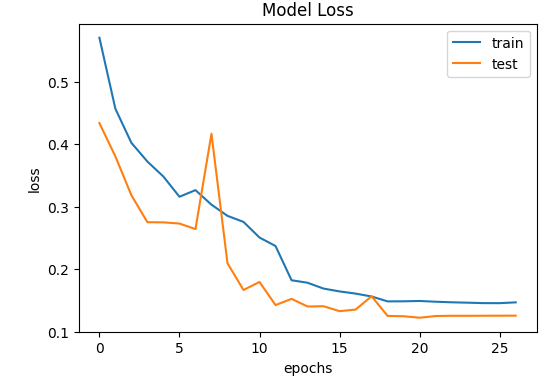
\includegraphics[width=0.60\textwidth]{4/figures/metadata_model_loss.png}
		\caption{Evolución de la pérdida de los subconjuntos de entrenamiento y validación para el modelo MLP de metadata para un entrenamiento de 100 épocas. Fuente: Elaboración propia.}
		\label{5:fig2}
	\end{center}
\end{figure}

La matriz de confusión resultante se representa en la Figura \ref{5:fig3}.

\begin{figure}[!ht]
	\begin{center}
		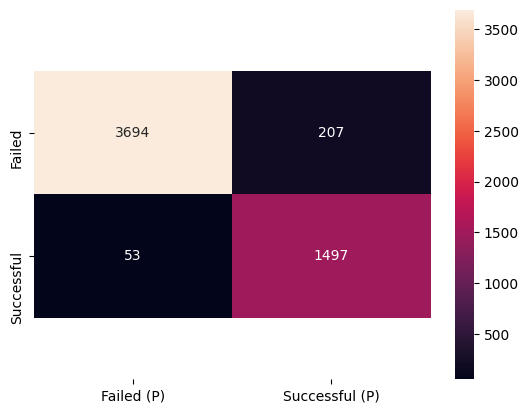
\includegraphics[width=0.60\textwidth]{4/figures/metadata_confusion_matrix.png}
		\caption{Matriz de confusión para el modelo de metadata. Fuente: Elaboración propia.}
		\label{5:fig3}
	\end{center}
\end{figure}

De esta matriz, derivan los resultados de la Tabla \ref{5:table1} evaluados según las métricas seleccionadas (citar).

\begin{table}[h!]
	\centering
	\small
	\begin{tabular}{ |m{4.5cm}|m{2.5cm}|m{2.5cm}|m{2.5cm}|m{2.5cm}|  }
		\hline
		\rowcolor{bluejean}
		\Centering \color{white}{Valor}& \Centering \color{white}{Precisión}& \Centering \color{white}{Sensibilidad}& \Centering \color{white}{Puntaje F1}& \Centering \color{white}{Muestras}\\
		\hline
		\textbf{Fracasado} & 0.99 & 0.95 & 0.97 & 3,901 \\
		\hline
		\textbf{Exitoso} & 0.88 & 0.97 & 0.92 & 1,550 \\
		\hline
		\rowcolor{turq}
		\multicolumn{5}{c}{ } \\
		\hline
		\textbf{Exactitud} &  &	 & 0.95 & 5,451 \\
		\hline
		\textbf{Promedio macro} & 0.93 & 0.96 & 0.94 & 5,451 \\
		\hline
		\textbf{Promedio ponderado} & 0.96 & 0.95 & 0.95 & 5,451 \\
		\hline
	\end{tabular}
	\caption{Informe de clasificación para el modelo de metadata. Fuente: Elaboración propia.}
	\label{5:table1}
\end{table}

Además, el área bajo la curva (AUC) tuvo un valor de como se muestra en la Figura \ref{5:fig4}.

\begin{figure}[!ht]
	\begin{center}
		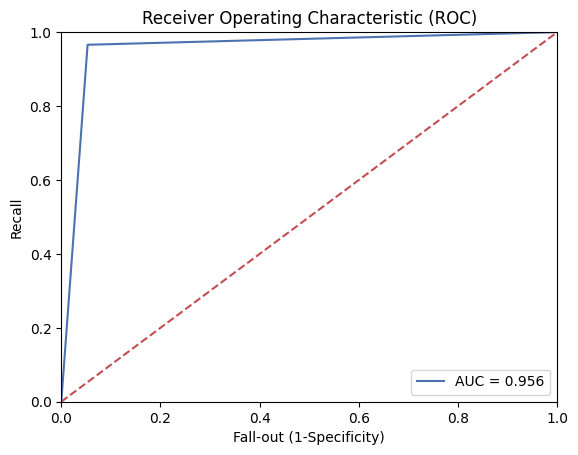
\includegraphics[width=0.60\textwidth]{4/figures/metadata_auc.png}
		\caption{Área bajo la curva de modelo de metadata. Fuente: Elaboración propia.}
		\label{5:fig4}
	\end{center}
\end{figure}

\section{Descripción}
Luego de 78 épocas, con un rango entre 102 y 114 segundos de entrenamiento cada una, el modelo dejó de entrenar dado que durante 10 épocas no registró una reducción en el valor de la pérdida del subconjunto de validación, por más que 5 épocas antes se había reducido su tasa de aprendizaje.

Así, de acuerdo a las Figuras \ref{5:fig5} y \ref{5:fig6}, en la época 68 se registran los mejores valores de exactitud y pérdida para el subconjunto de validación, alcanzando 0.7665 y 0.4922 respectivamente.

\begin{figure}[htbp]
	\begin{center}
		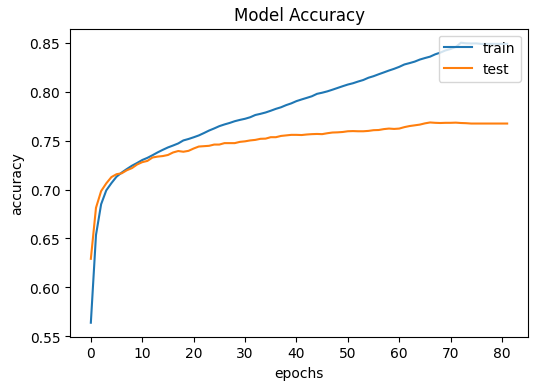
\includegraphics[width=0.60\textwidth]{4/figures/description_model_accuracy.png}
		\caption{Evolución de la exactitud de los subconjuntos de entrenamiento y validación para el modelo CNN de descripciones para un entrenamiento de 100 épocas. Fuente: Elaboración propia.}
		\label{5:fig5}
		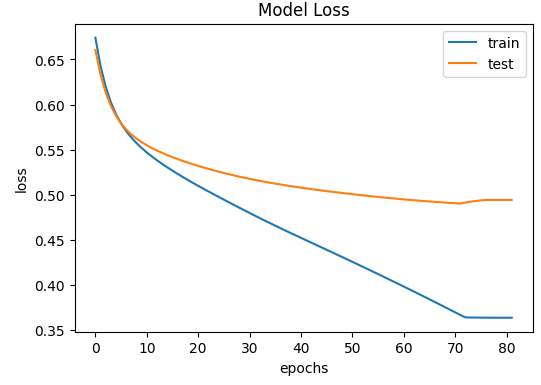
\includegraphics[width=0.60\textwidth]{4/figures/description_model_loss.png}
		\caption{Evolución de la pérdida de los subconjuntos de entrenamiento y validación para el modelo CNN de descripciones para un entrenamiento de 100 épocas. Fuente: Elaboración propia.}
		\label{5:fig6}
	\end{center}
\end{figure}

La matriz de confusión resultante se representa en la Figura \ref{5:fig7}.

\begin{figure}[!ht]
	\begin{center}
		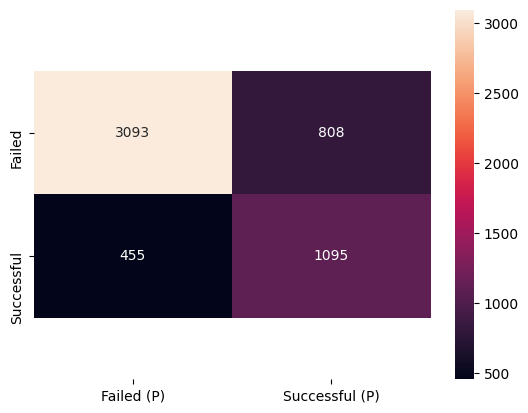
\includegraphics[width=0.60\textwidth]{4/figures/description_confusion_matrix.png}
		\caption{Matriz de confusión para el modelo de descripciones. Fuente: Elaboración propia.}
		\label{5:fig7}
	\end{center}
\end{figure}

De esta matriz, derivan los resultados de la Tabla \ref{5:table2} evaluados según las métricas seleccionadas (citar).

\begin{table}[h!]
	\centering
	\small
	\begin{tabular}{ |m{4.5cm}|m{2.5cm}|m{2.5cm}|m{2.5cm}|m{2.5cm}|  }
		\hline
		\rowcolor{bluejean}
		\Centering \color{white}{Valor}& \Centering \color{white}{Precisión}& \Centering \color{white}{Sensibilidad}& \Centering \color{white}{Puntaje F1}& \Centering \color{white}{Muestras}\\
		\hline
		\textbf{Fracasado} & 0.87 & 0.79 & 0.83 & 3,901 \\
		\hline
		\textbf{Exitoso} & 0.58 & 0.71 & 0.63 & 1,550 \\
		\hline
		\rowcolor{turq}
		\multicolumn{5}{c}{ } \\
		\hline
		\textbf{Exactitud} &  &	 & 0.77 & 5,451 \\
		\hline
		\textbf{Promedio macro} & 0.72 & 0.75 & 0.73 & 5,451 \\
		\hline
		\textbf{Promedio ponderado} & 0.79 & 0.77 & 0.77 & 5,451 \\
		\hline
	\end{tabular}
	\caption{Informe de clasificación para el modelo de descripciones. Fuente: Elaboración propia.}
	\label{5:table2}
\end{table}

Además, el área bajo la curva (AUC) tuvo un valor de como se muestra en la Figura \ref{5:fig8}.

\begin{figure}[!ht]
	\begin{center}
		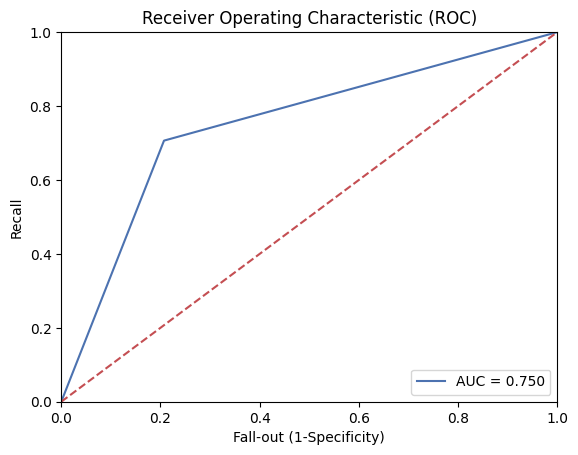
\includegraphics[width=0.60\textwidth]{4/figures/description_auc.png}
		\caption{Área bajo la curva de modelo de descripciones. Fuente: Elaboración propia.}
		\label{5:fig8}
	\end{center}
\end{figure}

\section{Comentarios}
Luego de 43 épocas, con 77 segundos en promedio de entrenamiento cada una, el modelo dejó de entrenar dado que durante 10 épocas no registró una reducción en el valor de la pérdida del subconjunto de validación, por más que 1 época antes se había reducido su tasa de aprendizaje.

Así, de acuerdo a las Figuras \ref{5:fig9} y \ref{5:fig10}, en la época 33 se registran los mejores valores de exactitud y pérdida para el subconjunto de validación, alcanzando 0.8510 y 0.4472 respectivamente.

\begin{figure}[htbp]
	\begin{center}
		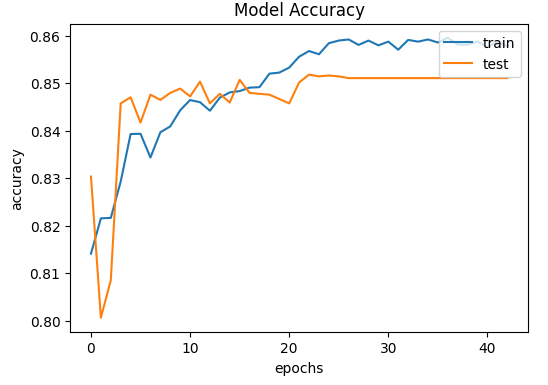
\includegraphics[width=0.60\textwidth]{4/figures/comments_model_accuracy.png}
		\caption{Evolución de la exactitud de los subconjuntos de entrenamiento y validación para el modelo RNN de comentarios para un entrenamiento de 50 épocas. Fuente: Elaboración propia.}
		\label{5:fig9}
		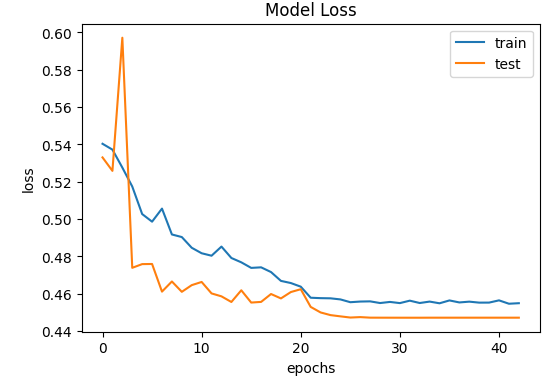
\includegraphics[width=0.60\textwidth]{4/figures/comments_model_loss.png}
		\caption{Evolución de la pérdida de los subconjuntos de entrenamiento y validación para el modelo RNN de comentarios para un entrenamiento de 50 épocas. Fuente: Elaboración propia.}
		\label{5:fig10}
	\end{center}
\end{figure}

La matriz de confusión resultante se representa en la Figura \ref{5:fig11}.
\begin{figure}[!ht]
	\begin{center}
		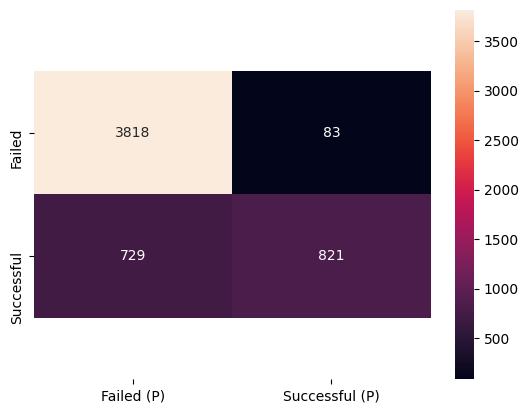
\includegraphics[width=0.60\textwidth]{4/figures/comments_confusion_matrix.png}
		\caption{Matriz de confusión para el modelo de comentarios. Fuente: Elaboración propia.}
		\label{5:fig11}
	\end{center}
\end{figure}

De esta matriz, derivan los resultados de la Tabla \ref{5:table3} evaluados según las métricas seleccionadas (citar).

\begin{table}[h!]
	\centering
	\small
	\begin{tabular}{ |m{4.5cm}|m{2.5cm}|m{2.5cm}|m{2.5cm}|m{2.5cm}|  }
		\hline
		\rowcolor{bluejean}
		\Centering \color{white}{Valor}& \Centering \color{white}{Precisión}& \Centering \color{white}{Sensibilidad}& \Centering \color{white}{Puntaje F1}& \Centering \color{white}{Muestras}\\
		\hline
		\textbf{Fracasado} & 0.84 & 0.98 & 0.90 & 3,901 \\
		\hline
		\textbf{Exitoso} & 0.91 & 0.53 & 0.67 & 1,550 \\
		\hline
		\rowcolor{turq}
		\multicolumn{5}{c}{ } \\
		\hline
		\textbf{Exactitud} &  &	 & 0.85 & 5,451 \\
		\hline
		\textbf{Promedio macro} & 0.87 & 0.75 & 0.79 & 5,451 \\
		\hline
		\textbf{Promedio ponderado} & 0.86 & 0.85 & 0.84 & 5,451 \\
		\hline
	\end{tabular}
	\caption{Informe de clasificación para el modelo de comentarios. Fuente: Elaboración propia.}
	\label{5:table3}
\end{table}

Además, el área bajo la curva (AUC) tuvo un valor de como se muestra en la Figura \ref{5:fig12}.

\begin{figure}[!ht]
	\begin{center}
		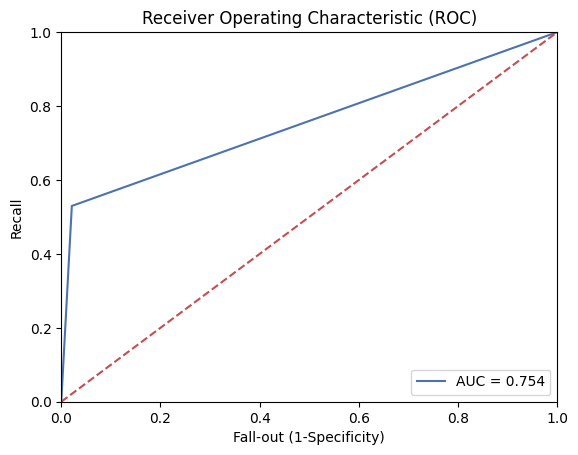
\includegraphics[width=0.60\textwidth]{4/figures/comments_auc.png}
		\caption{Área bajo la curva de modelo de comentarios. Fuente: Elaboración propia.}
		\label{5:fig12}
	\end{center}
\end{figure}

\section{Modelo apilado}
Luego de 13 épocas, con 152 segundos en promedio de entrenamientos cada una, el modelo dejó de entrenar dado que durante 10 épocas no registró una reducción en el valor de la pérdida del subconjunto de validación, por más que 2 épocas antes se había reducido su tasa de aprendizaje.

Así, de acuerdo a las Figuras \ref{5:fig13} y \ref{5:fig14}, en la época 3 se registran los mejores valores de exactitud y pérdida para el subconjunto de validación, alcanzando 0.9336 y 0.1810 respectivamente.

\begin{figure}[htbp]
	\begin{center}
		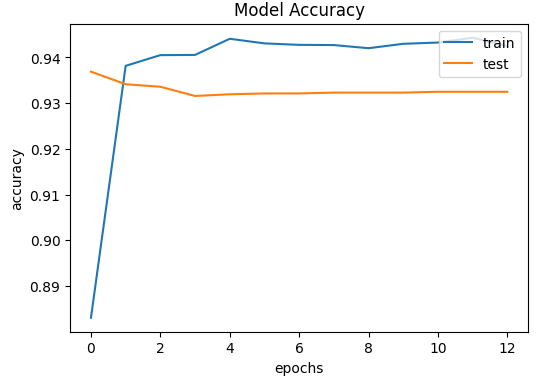
\includegraphics[width=0.60\textwidth]{4/figures/stacked_model_accuracy.png}
		\caption{Evolución de la exactitud de los subconjuntos de entrenamiento y validación para el modelo apilado para un entrenamiento de 200 épocas. Fuente: Elaboración propia.}
		\label{5:fig13}
		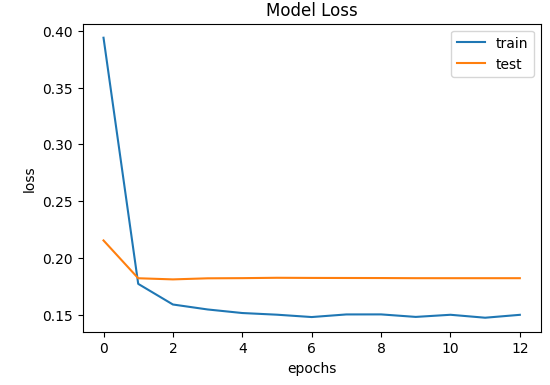
\includegraphics[width=0.60\textwidth]{4/figures/stacked_model_loss.png}
		\caption{Evolución de la pérdida de los subconjuntos de entrenamiento y validación para el modelo apilado para un entrenamiento de 200 épocas. Fuente: Elaboración propia.}
		\label{5:fig14}
	\end{center}
\end{figure}

La matriz de confusión resultante se representa en la Figura \ref{5:fig15}.
\begin{figure}[!ht]
	\begin{center}
		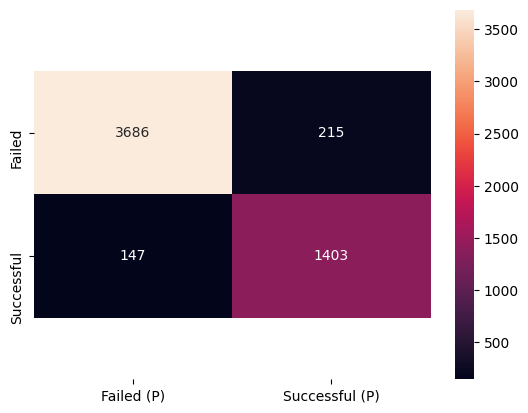
\includegraphics[width=0.60\textwidth]{4/figures/stacked_confusion_matrix.png}
		\caption{Matriz de confusión para el modelo apilado. Fuente: Elaboración propia.}
		\label{5:fig15}
	\end{center}
\end{figure}

De esta matriz, derivan los resultados de la Tabla \ref{5:table4} evaluados según las métricas seleccionadas (citar).

\begin{table}[h!]
	\centering
	\small
	\begin{tabular}{ |m{4.5cm}|m{2.5cm}|m{2.5cm}|m{2.5cm}|m{2.5cm}|  }
		\hline
		\rowcolor{bluejean}
		\Centering \color{white}{Valor}& \Centering \color{white}{Precisión}& \Centering \color{white}{Sensibilidad}& \Centering \color{white}{Puntaje F1}& \Centering \color{white}{Muestras}\\
		\hline
		\textbf{Fracasado} & 0.96 & 0.94 & 0.95 & 3,901 \\
		\hline
		\textbf{Exitoso} & 0.87 & 0.91 & 0.89 & 1,550 \\
		\hline
		\rowcolor{turq}
		\multicolumn{5}{c}{ } \\
		\hline
		\textbf{Exactitud} &  &	 & 0.93 & 5,451 \\
		\hline
		\textbf{Promedio macro} & 0.91 & 0.93 & 0.92 & 5,451 \\
		\hline
		\textbf{Promedio ponderado} & 0.93 & 0.93 & 0.93 & 5,451 \\
		\hline
	\end{tabular}
	\caption{Informe de clasificación para el modelo apilado. Fuente: Elaboración propia.}
	\label{5:table4}
\end{table}

Además, el área bajo la curva (AUC) tuvo un valor de como se muestra en la Figura \ref{5:fig16}.

\begin{figure}[!ht]
	\begin{center}
		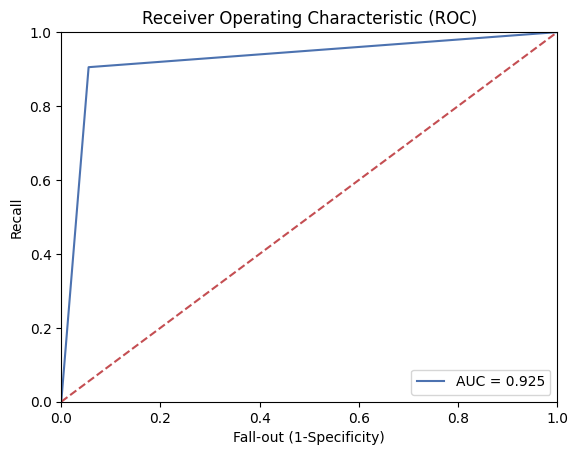
\includegraphics[width=0.60\textwidth]{4/figures/stacked_auc.png}
		\caption{Área bajo la curva de modelo apilado. Fuente: Elaboración propia.}
		\label{5:fig16}
	\end{center}
\end{figure}

\section{Demostración del modelo final}